\section{Figure Captions}

\textbf{Figure~\ref{fig:domain_proxy}} (\texttt{fig1\_domain\_proxy\_comparison.png}): Bar chart showing mean entity density, narrative coherence, and formal syntax density for all 21 Pile domains. Wikipedia shows highest entity density; BookCorpus2 shows highest narrative coherence; GitHub shows highest formal syntax density. Error bars show 95\% confidence intervals.

\textbf{Figure~\ref{fig:focal_violins}} (\texttt{fig2\_focal\_violins.png}): Violin plots comparing the three focal domains (Wikipedia, BookCorpus2, GitHub) across all three cognitive proxies.

\begin{figure}[h]
\centering
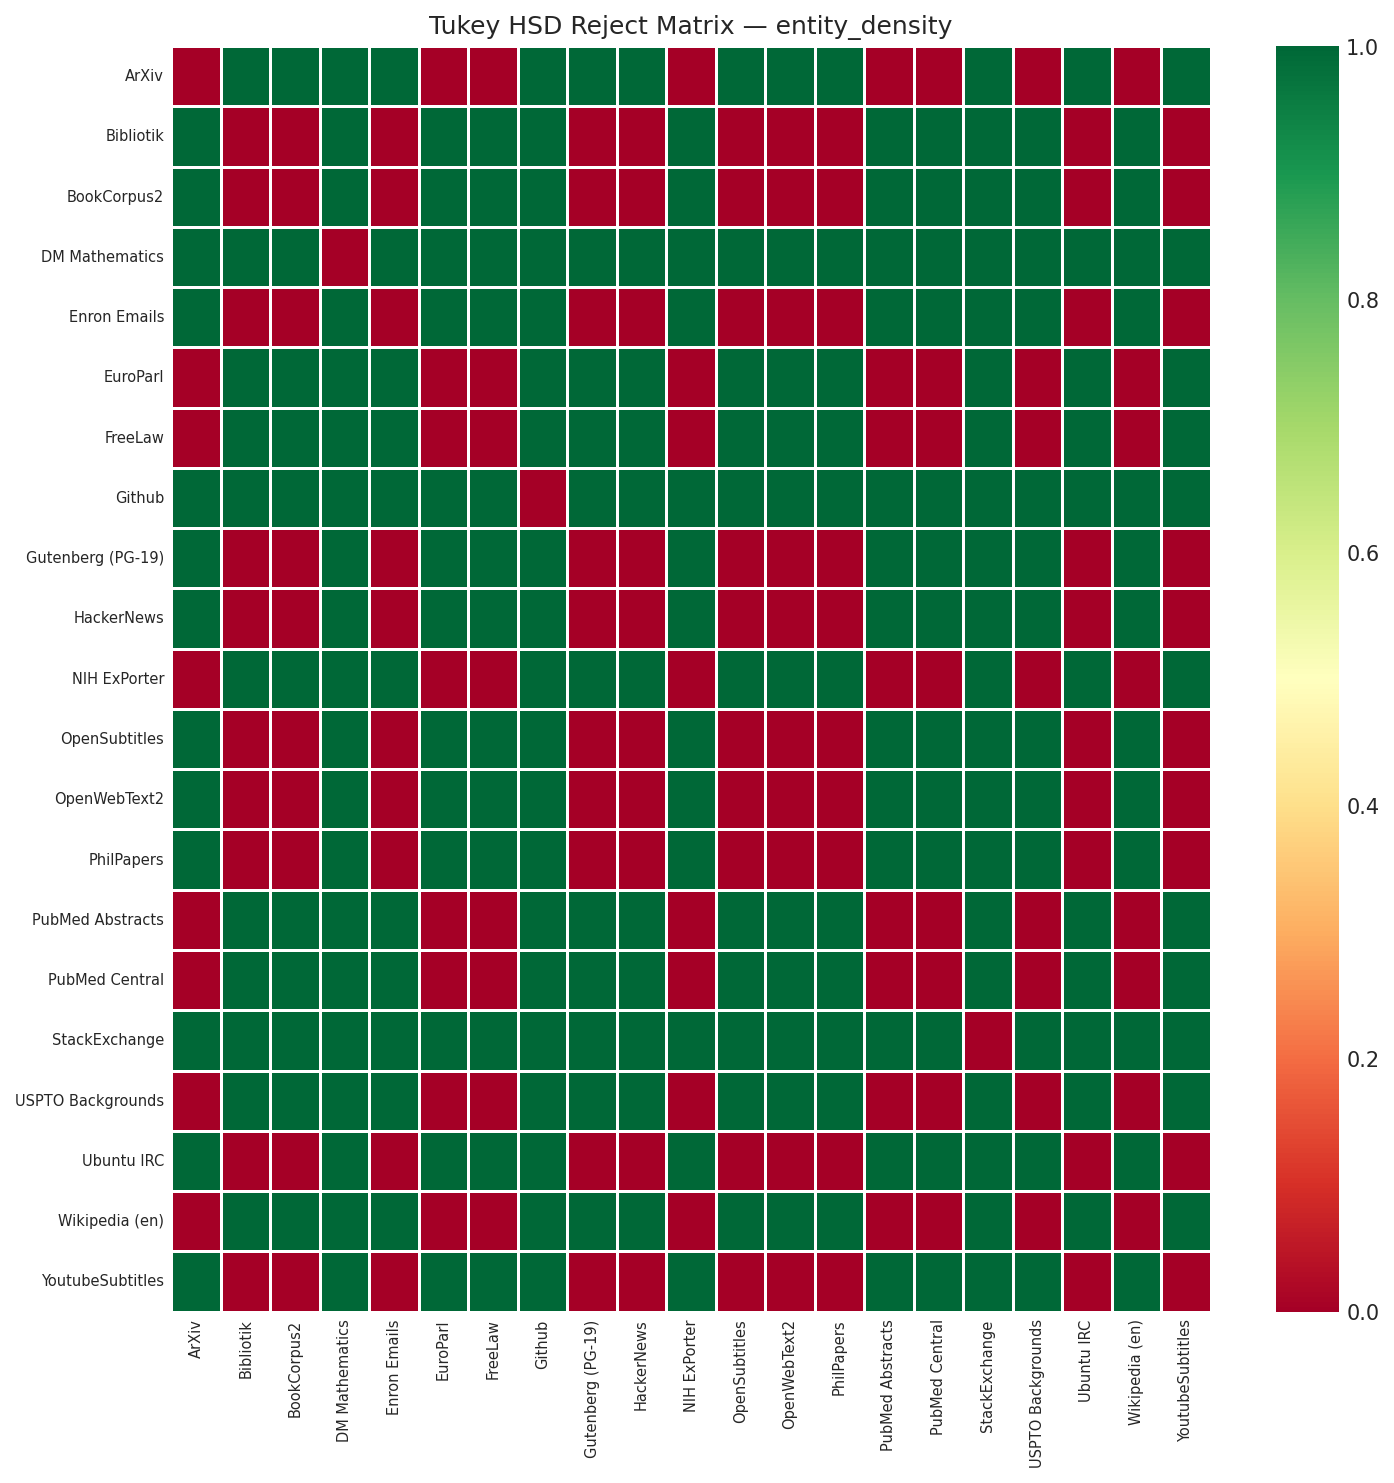
\includegraphics[width=\linewidth]{figures/fig3_tukey_heatmap.png}
\caption{21$\times$21 Tukey HSD reject matrix for entity density. Dark cells indicate significant pairwise differences ($p < 0.001$). Wikipedia-vs-Books and GitHub-vs-all comparisons are among the most significant.}
\label{fig:tukey}
\end{figure}

\begin{figure}[h]
\centering
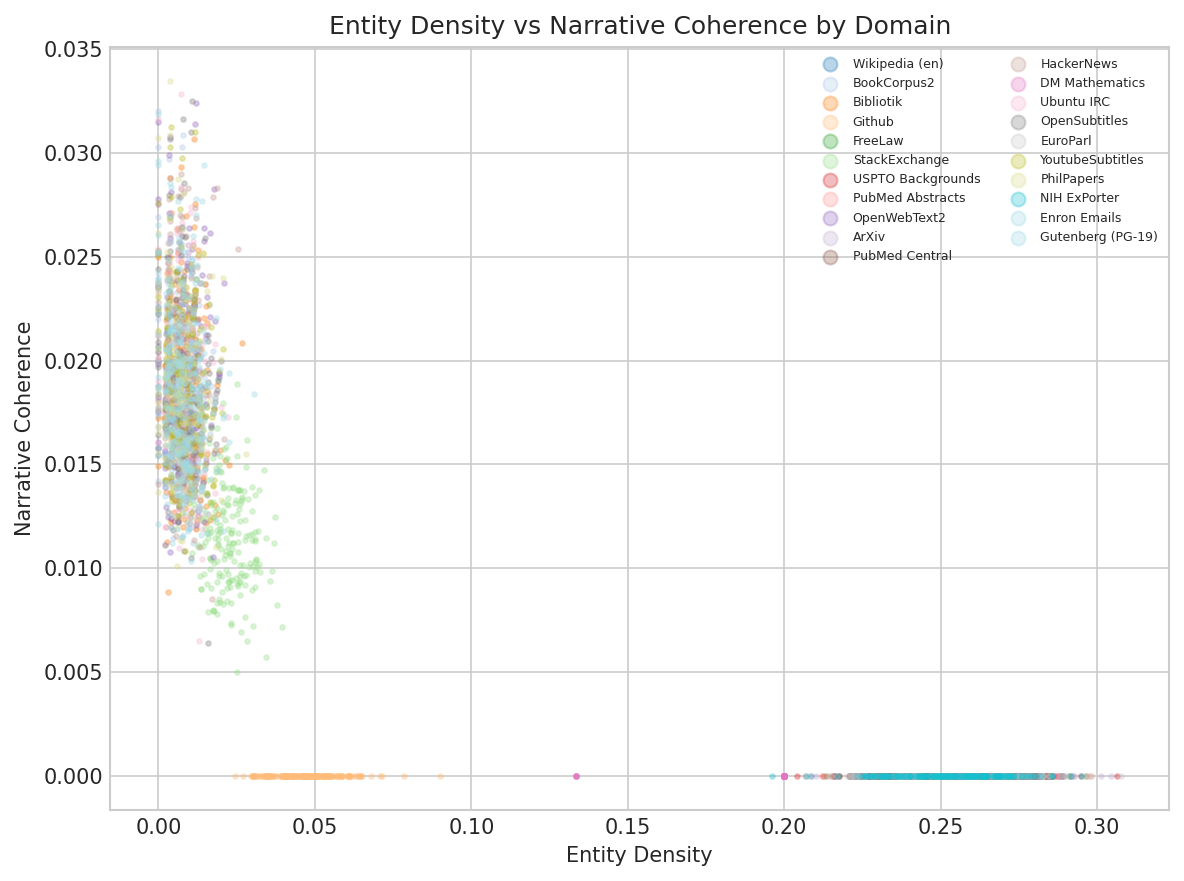
\includegraphics[width=\linewidth]{figures/fig4_proxy_scatter.png}
\caption{Scatter plot of narrative coherence vs entity density for all documents, colored by domain. Clear clustering confirms that domains occupy distinct regions of the cognitive proxy space.}
\label{fig:scatter}
\end{figure}

\begin{figure}[h]
\centering
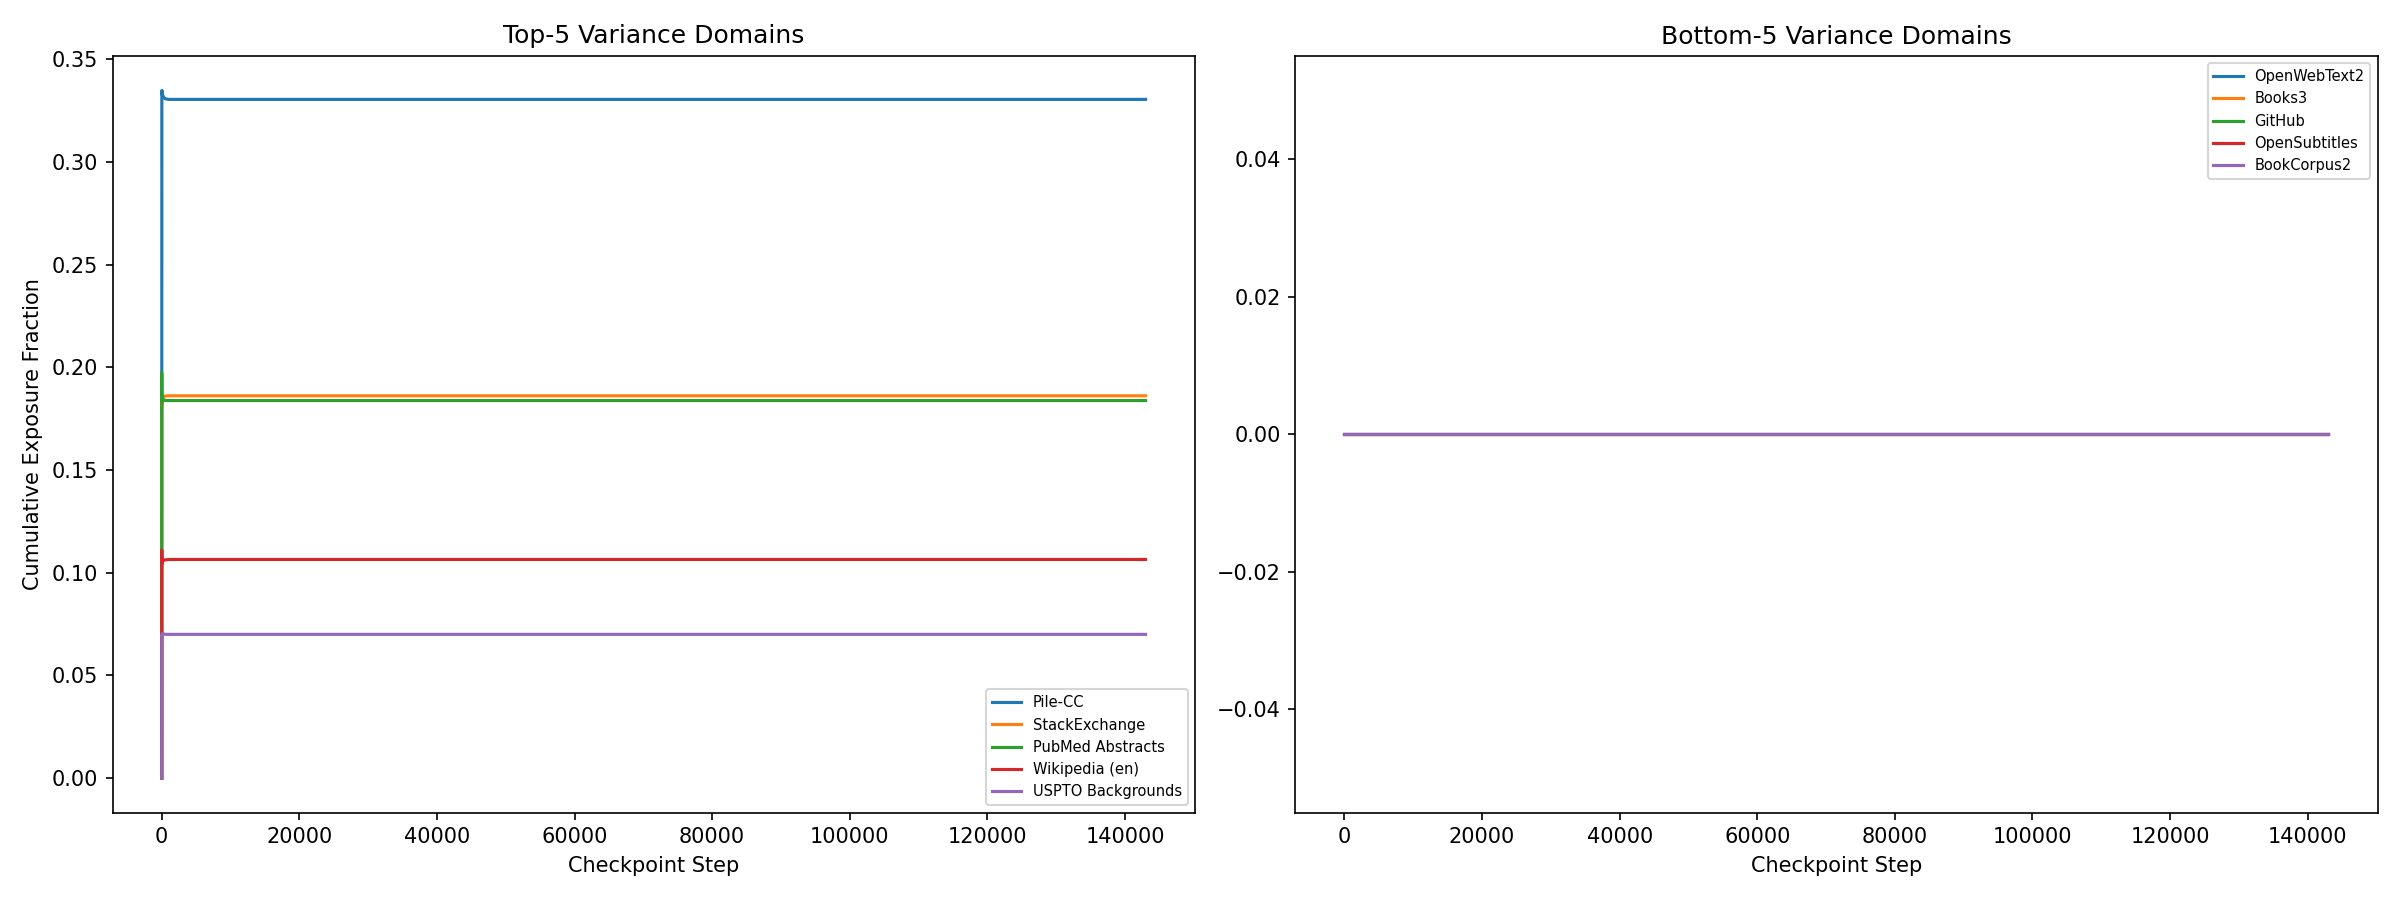
\includegraphics[width=\linewidth]{figures/trajectories.png}
\caption{Cumulative domain exposure fraction trajectories for the top-5 and bottom-5 variance domains across all 154 training checkpoints. High-variance domains show monotonic but non-uniform growth; zero-variance domains are flat at 0.0.}
\label{fig:trajectories}
\end{figure}

\begin{figure}[h]
\centering
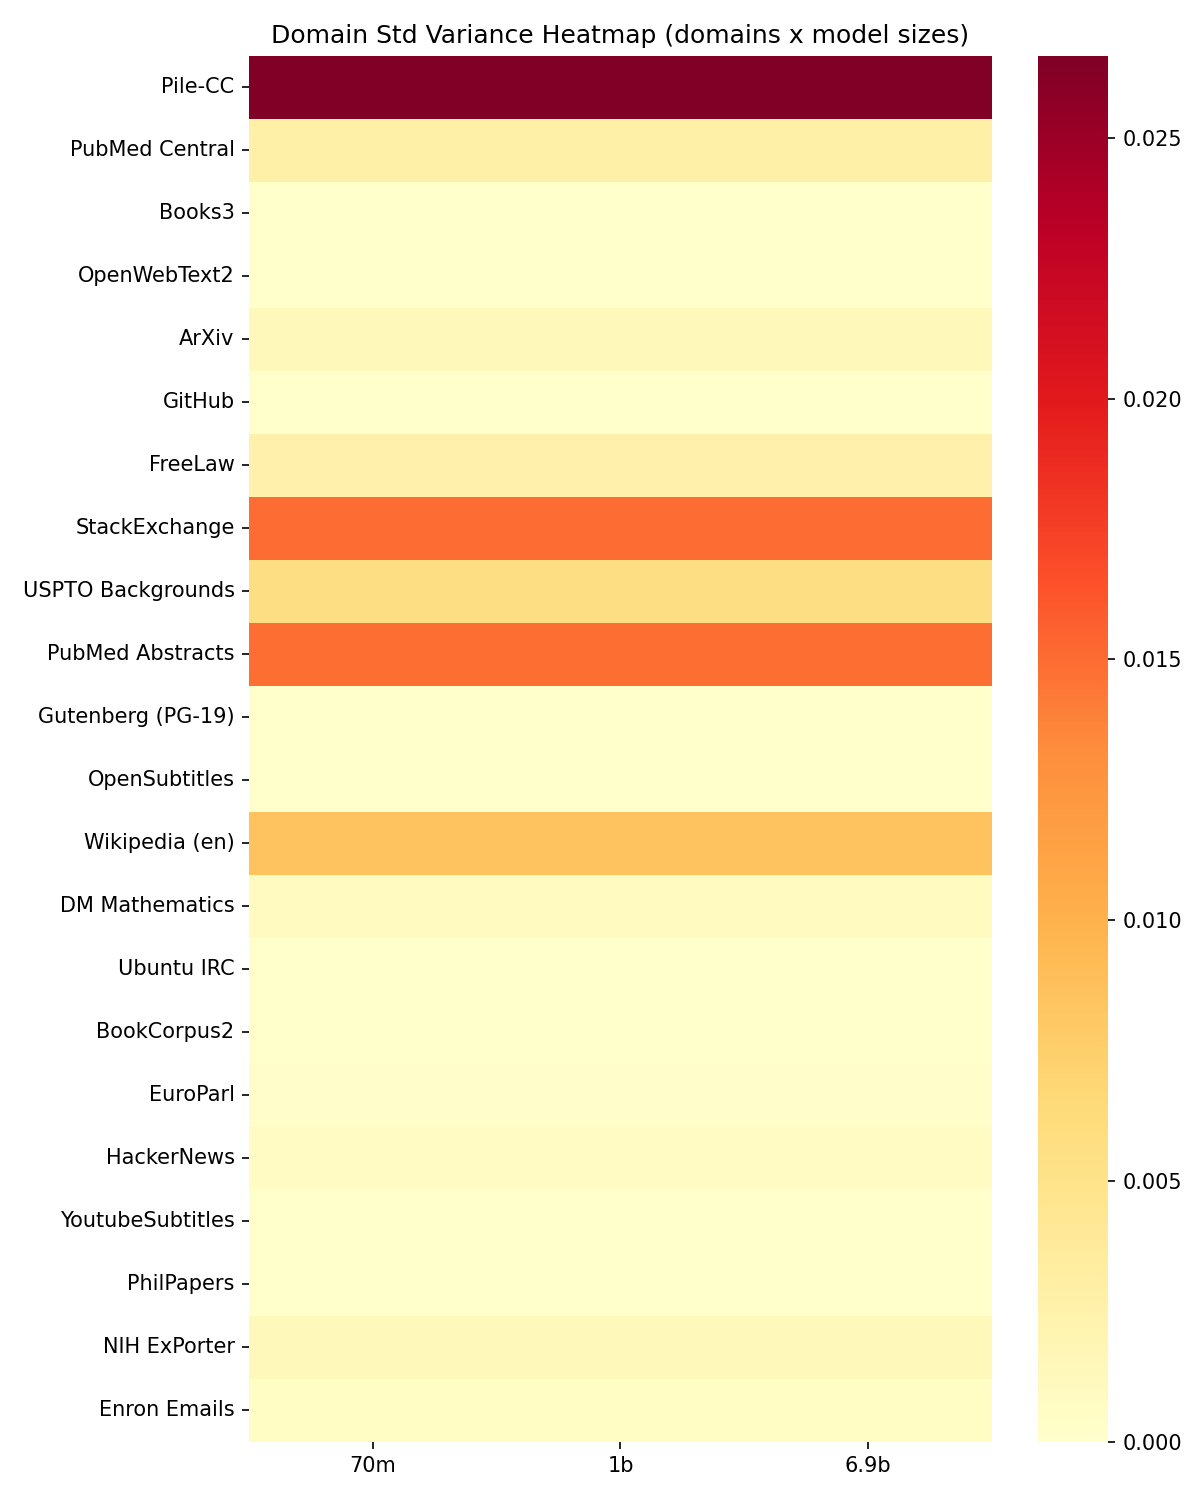
\includegraphics[width=\linewidth]{figures/variance_heatmap.png}
\caption{Heatmap of per-domain trajectory standard deviation for all 22 domains $\times$ 3 model sizes (70M, 1B, 6.9B). Near-identical columns confirm that domain exposure trajectories are determined by data ordering, not model-specific dynamics.}
\label{fig:variance_heatmap}
\end{figure}

\begin{figure}[h]
\centering
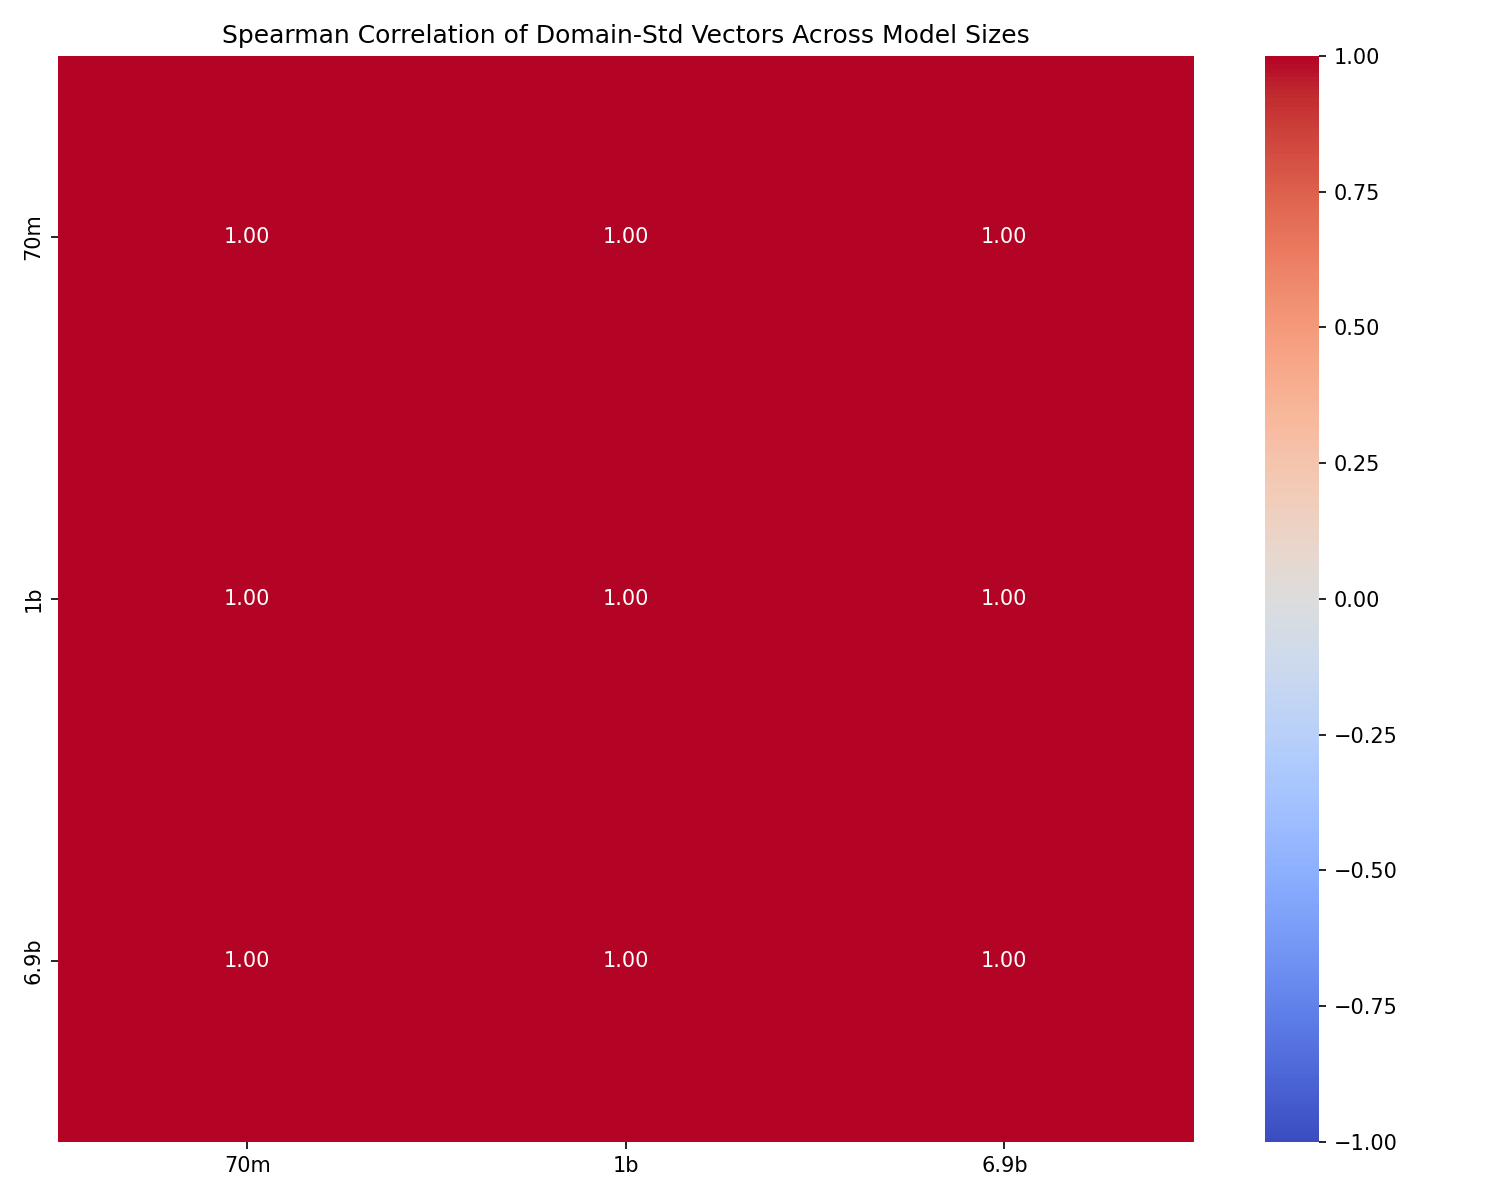
\includegraphics[width=\linewidth]{figures/spearman_matrix.png}
\caption{Spearman correlation matrix between domain exposure trajectories across the three model sizes. Near-unity correlations confirm cross-scale consistency.}
\label{fig:spearman_matrix}
\end{figure}
